\section{System Calls}
\subsection{Aim}
To familiarize and understand the use and functioning of System Calls used for Operating
system and network programming in Linux.
\subsection{Theory}
\subsubsection{Process Control}
\begin{enumerate}
	\item \textbf{fork()} \\
	The fork() function creates child processes. It takes no arguments and returns
	the 0 for the child process and process ID of the child to the parent process. child
	process starts executing from the next instruction after fork.

	Function synopsis:
	\begin{lstlisting}[language=C]
#include <unistd.h>
pid_t fork(void);
	\end{lstlisting}

	\item \textbf{getpid()} \\
	It returns the process ID of the calling process

	Function synopsis:
	\begin{lstlisting}[language=C]
#include <unistd.h>
pid_t getpid(void);
	\end{lstlisting}

	\item \textbf{exit()} \\
	The exit() function terminates the calling processes. Child processes of the calling
	process will be inherited by process \#1 (init) and the parent process which spawned the
	calling process is sent a SIGCHILD signal

	Function synopsis:
	\begin{lstlisting}[language=C]
#include <stdlib.h>
void exit(int status);
	\end{lstlisting}

	The status can be EXIT\_FAILURE or EXIT\_SUCCESS

	\item \textbf{wait()} \\
	The wait() function puts the calling process to waiting state until the child process of
	it terminates. It takes a integer pointer where the exit status of the child process will 
	be stored and returns the process ID of the child process that terminated.

	Function synopsis:
	\begin{lstlisting}[language=C]
#include <sys/wait.h>
pid_t wait(int *stat_loc);
	\end{lstlisting}
\end{enumerate}


\subsubsection{File Manipulation}
\begin{enumerate}
	\item \textbf{open()} \\
	The open() function establishes a connection between a file and a file descriptor. It creates and
	open file description and returns the file descriptor corresponding to the description. This file 
	descriptor can be used for the I/O operations on the file

	Function synopsis:
	\begin{lstlisting}[language=C]
#include <sys/stat.h>
#include <fcntl.h>
int open(const char *path, int oflag, ...);
	\end{lstlisting}

	\item \textbf{close()} \\
	It delocates the file descriptor so that it can be reused for other files. Any locks obtained by the 
	process on that file is removed. If this was the last file descriptor to point to an open file description
	then the file description is removed from memory

	Function synopsis:
	\begin{lstlisting}[language=C]
#include <unistd.h>
int getpid(int fd);
	\end{lstlisting}

	\item \textbf{read()} \\
	The read() function reads from the file descriptor. read() attempts to read up to count bytes from 
	file descriptor fd into the buffer starting at buf. On success, number of bytes read is returned. On error
	-1 is returned and errno is set.

	Function synopsis:
	\begin{lstlisting}[language=C]
#include <unistd.h>
ssize_t read(int fd, void *buf, size_t count);
	\end{lstlisting}

	The status can be EXIT\_FAILURE or EXIT\_SUCCESS

	\item \textbf{write()} \\
	The wait() function puts the calling process to waiting state until the child process of
	it terminates. It takes a integer pointer where the exit status of the child process will 
	be stored and returns the process ID of the child process that terminated.

	Function synopsis:
	\begin{lstlisting}[language=C]
#include <sys/wait.h>
pid_t wait(int *stat_loc);
	\end{lstlisting}
\end{enumerate}


\subsubsection{Device Manipulation}
\begin{enumerate}
	\item \textbf{ioctl()} \\
	The ioctl() function is used to control a stream device. It is a device-specific system call 
	used for terminal I/O, hardware device control, and kernel extension operations. It returns 0
	for success and -1 for error.

	Function synopsis:
	\begin{lstlisting}[language=C]
include <stropts.h>
int ioctl(int fd, int request, ... /* arg */); 
	\end{lstlisting}

	\item \textbf{read()} \\
	Same as in File Manipulation

	\item \textbf{write()} \\
	Same as in File Manipulation
\end{enumerate}


\subsubsection{Information Maintenance}
\begin{enumerate}
	\item \textbf{alarm()} \\
	It is used to schedule an alarm. The calling process will recieve
	SIGALRM signal after seconds provided as argument.

	Function synopsis:
	\begin{lstlisting}[language=C]
#include <unistd.h>
unsigned alarm(unsigned seconds);
	\end{lstlisting}

	\item \textbf{sleep()} \\
	Suspends the execution of calling process for an interval of time specified
	by the parameter passed

	Function synopsis:
	\begin{lstlisting}[language=C]
#include <unistd.h>
unsigned sleep(unsigned seconds);
	\end{lstlisting}

	\item \textbf{getpid()} \\
	Same as in Process Control
\end{enumerate}


\subsubsection{Interprocess Communication}
\begin{enumerate}
	\item \textbf{pipe()} \\
	The pipe() function establishes a interprocess channel. It takes a two element integer array To
	store the read and write ends of the pipe respectively

	Function synopsis:
	\begin{lstlisting}[language=C]
#include <unistd.h>
int pipe(int fd[2]);
	\end{lstlisting}

	\item \textbf{shmget()} \\
	It requests for a shared memory segment

	Function synopsis:
	\begin{lstlisting}[language=C]
#include <sys/shm.h>
int shmget(key_t key, size_t size, int shmflg)
	\end{lstlisting}
\end{enumerate}


\subsection{Source Code}
\subsubsection{Process Control}
\begin{lstlisting}[language=C]
#include <stdio.h>
#include <stdlib.h>
#include <unistd.h>
#include <sys/wait.h>

int main() {
	pid_t pid;

	if(fork() == 0) {
		pid = getpid();
		printf("PID of the child process is %d\n", pid);
		exit(EXIT_SUCCESS);
	} 

	pid = getpid();
	printf("PID of the parent process is %d\n", pid);
	printf("Parent going to wait state\n");
	wait(NULL);
	printf("Parent executing after termination of child\n");

	return 0;
}
\end{lstlisting}

\begin{center}
	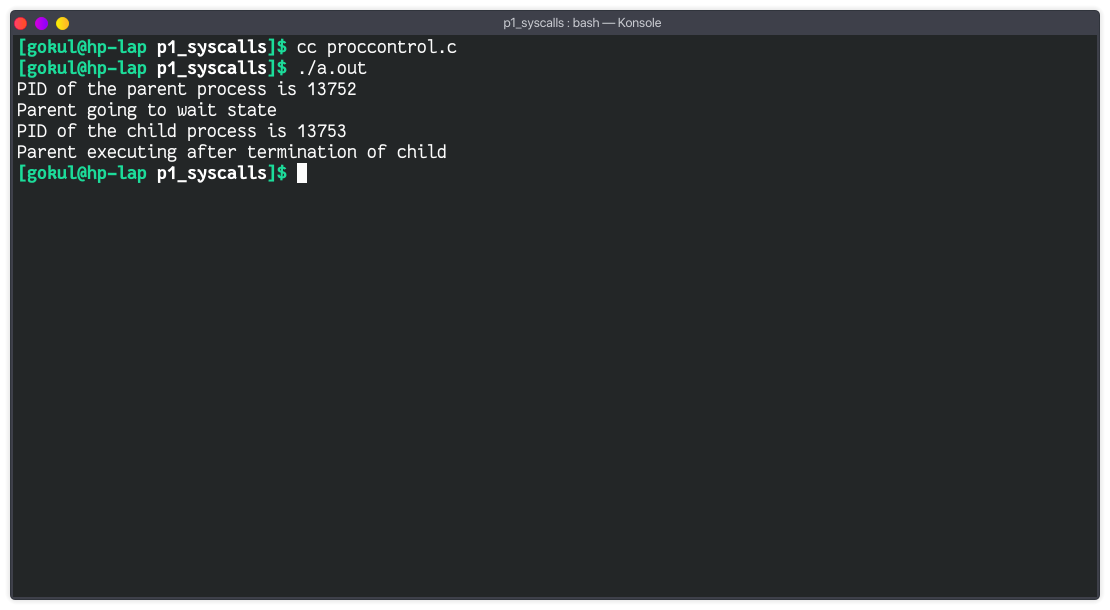
\includegraphics[width=0.90\textwidth]{img/p2/ss1.png}
\end{center}

\subsubsection{File Manipulation}
\begin{lstlisting}[language=C]
#include <stdio.h>
#include <stdlib.h>
#include <string.h>
#include <sys/types.h>
#include <sys/stat.h>
#include <fcntl.h>
#include <unistd.h>
#include <errno.h>

extern int errno;

int main() {
	int fd = open("file.txt", O_WRONLY | O_CREAT);
	char text_to_write[] = "Hello world";
	char *text_read = malloc(512 * sizeof(char));
	
	if(fd == -1) {
		printf("File open failed with error code %d\n", errno);
		exit(1);
	}

	printf("File descriptor for write #%d\n", fd);

	printf("Writing to file");
	write(fd, text_to_write, strlen(text_to_write));
	printf(" SUCCESS\n");

	close(fd);
	printf("Closed file\n");

	fd = open("file.txt", O_RDONLY);

	if(fd == -1) {
		printf("File open failed with error code %d\n", errno);
		exit(1);
	}

	printf("File descriptor for read #%d\n", fd);

	printf("Reading from file\n");
	read(fd, text_read, sizeof(text_to_write));
	printf("%s", text_read);

	close(fd);
	printf("\n");

	return 0;
}
\end{lstlisting}

\begin{center}
	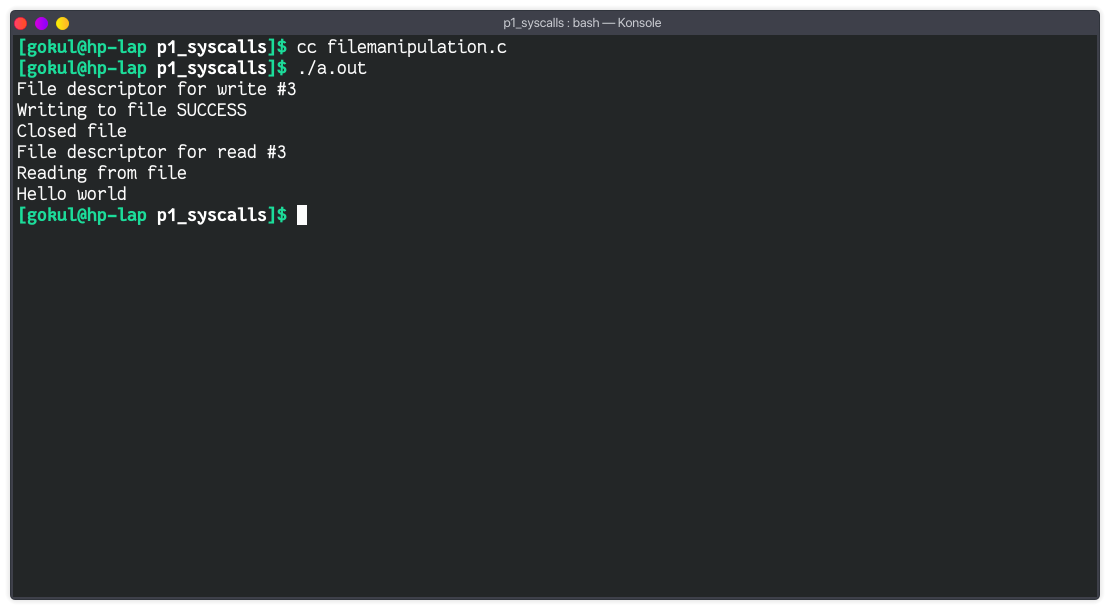
\includegraphics[width=0.90\textwidth]{img/p2/ss2.png}
\end{center}

\subsubsection{Information Maintenance}
\begin{lstlisting}[language=C]
#include <stdio.h>
#include <unistd.h>
#include <signal.h>
#include <sys/types.h>

void signal_handler() {
	printf("Timed out!\n");
}

int main() {
	unsigned int timeout, elapsed = 0;
	pid_t pid;

	pid = getpid();
	printf("The PID of the process is: %d\n", pid);

	printf("Set timeout after: ");
	scanf("%d", &timeout);

	signal(SIGALRM, signal_handler);
	alarm(timeout);

	while(elapsed++ < timeout) {
		printf("Sleeping for 1 second...\n");
		sleep(1);
	}

	return 0;
}		
\end{lstlisting}

\begin{center}
	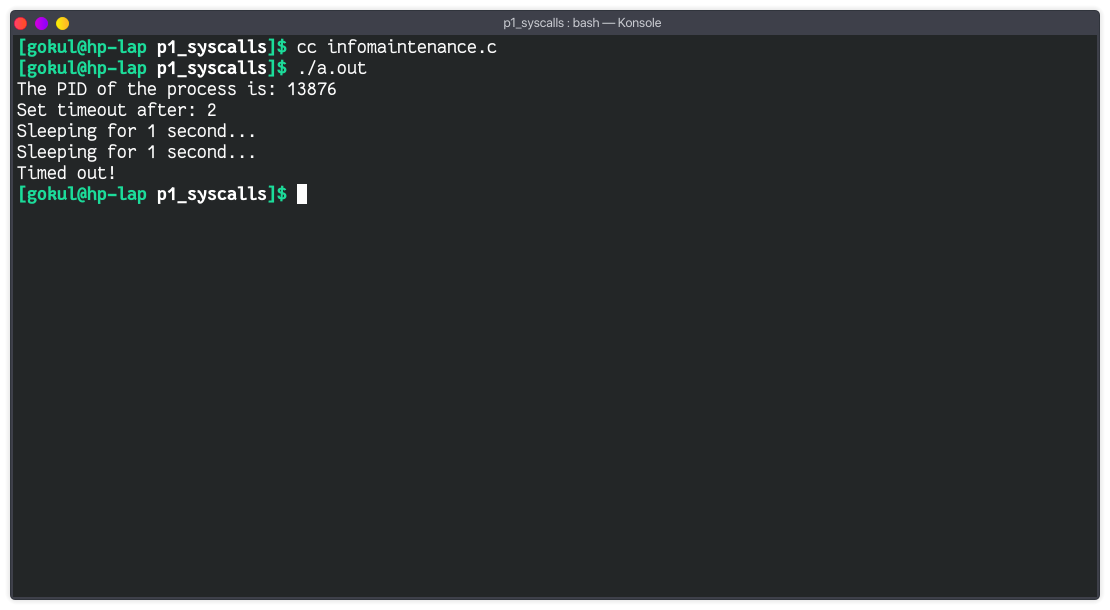
\includegraphics[width=0.90\textwidth]{img/p2/ss3.png}
\end{center}

\subsubsection{Interprocess Communication}
\begin{lstlisting}[language=C]
#include <stdio.h>
#include <stdlib.h>
#include <unistd.h>
#include <sys/types.h>
#include <sys/ipc.h>
#include <sys/shm.h>
#include <string.h>
#include <math.h>
#include <wait.h>

#define MESSAGE_LENGTH 6
#define FTOK_FILE "shmfile"

// Write to pipe
void pipe_write(int *pipe_fd, char *message) {
	printf("Writing to pipe");
	close(pipe_fd[0]); // Closing the read pipe
	write(pipe_fd[1], message, MESSAGE_LENGTH);
	printf(" SUCCESS\n");

	sleep(1);
	exit(EXIT_SUCCESS);
}

// Reads MESSAGE_LENGTH characters from pipe
void pipe_read(int *pipe_fd) {
	char message[10];

	wait(NULL); // Wait for pipe_write process to complete

	printf("Reading from pipe\n");
	close(pipe_fd[1]); // Closing the write pipe
	read(pipe_fd[0], message, MESSAGE_LENGTH);
	close(pipe_fd[0]); // Closing the read pipe

	printf("The message is: %s\n", message);

	exit(EXIT_SUCCESS);
}

// Write to shared memory segment
void shmget_write(char *message) {
	key_t key;
	int shm_id;
	
	key = ftok(FTOK_FILE, 'A'); // Generate a unique token
	shm_id = shmget(key, MESSAGE_LENGTH, 0666 | IPC_CREAT);

	printf("Writing message to shared memory segment");
	char *message_addr = 
		(char *) shmat(shm_id, (void *)0, 0); // Attach to shared memory
	strcpy(message_addr, message);
	shmdt(message_addr); // Detach from shared memory
	printf(" SUCCESS\n");

	sleep(1);
	exit(EXIT_SUCCESS);
}

// Read from shared memory
void shmget_read() {
	key_t key;
	int shm_id;
	char *message_addr;
	
	wait(NULL);

	key = ftok(FTOK_FILE, 'A'); // Generate a unique token
	shm_id = shmget(key, MESSAGE_LENGTH, 0666 | IPC_CREAT);

	printf("Reading message from shared memory segment\n");
	message_addr = (char *) shmat(shm_id, (void *)0, 0);
	printf("Message read is: %s\n", message_addr);
	shmdt(message_addr);

	shmctl(shm_id, IPC_RMID, NULL);
	exit(EXIT_SUCCESS);
}

// Process to facilitate pipe working
void pipe_process(char *message) {
	int pipe_fd[2];

	if(pipe(pipe_fd) == -1) {
		printf("Error in creating pipe\n");
		exit(EXIT_FAILURE);
	}

	if(fork() == 0) pipe_write(pipe_fd, message);

	pipe_read(pipe_fd);
}

// Function to facilitate Shared memory segment
void shmget_process(char *message) {
	wait(NULL); // Wait for pipe_process to stop

	if(fork() == 0) shmget_write(message);

	shmget_read();
}

int main() {
	char *message = "Hello";

	if(fork() == 0) pipe_process(message);

	shmget_process(message);

	return 0;
}
\end{lstlisting}

\begin{center}
	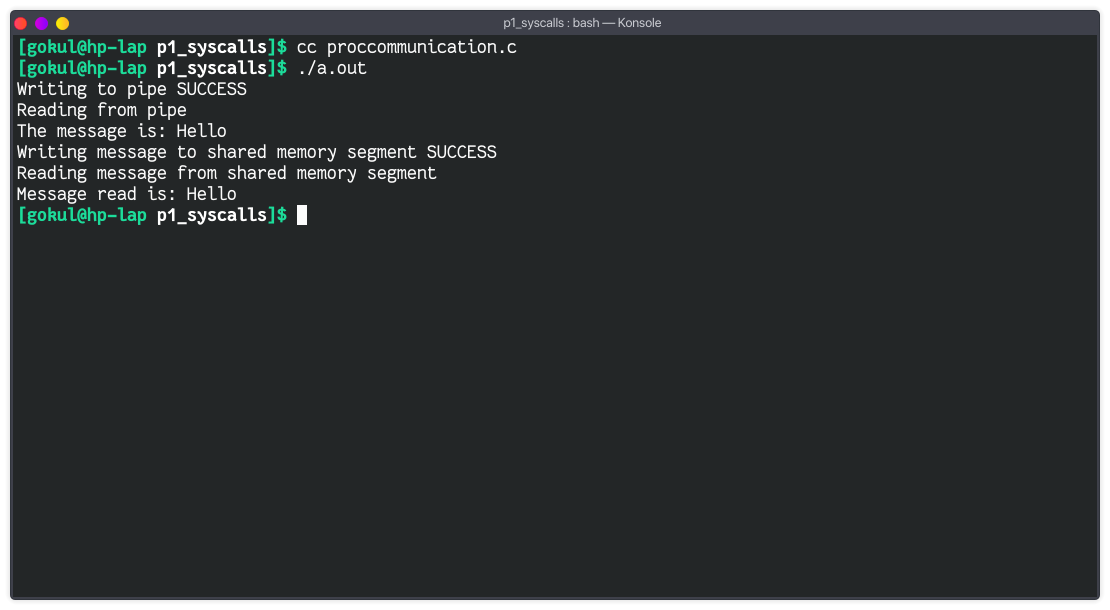
\includegraphics[width=0.90\textwidth]{img/p2/ss4.png}
\end{center}

\subsection{Result}
The above programs were executed and their outputs were verified